\documentclass[english,fleqn,allpages]{ISTE_science}[2018/07/30]


\setcounter{MaxMatrixCols}{30}
\usepackage{amsthm}
%\usepackage{OKS_ISTE}
%\CropMarksOn
\usepackage{natbib}
\renewcommand\bibsection{\section{\bibname}}
\setlength{\bibsep}{3pt} 
\makeatletter

%\newcounter{numdef}[chapter] \global\long\def\thenumdef{\thechapter.\arabic{numdef}}
% \global\long\def\NumberedDefinition#1


\newsavebox{\fminibox} \newlength{\fminilength} \newenvironment{fminipage}[1][\linewidth]{%
 \setlength{\fminilength}{#1 - 2\fboxsep - 2\fboxrule}
 \begin{lrbox}{\fminibox}
  \begin{minipage}{\fminilength}}{%
  \end{minipage}
 \end{lrbox}
 \noindent
 \fbox{\usebox{\fminibox}}}


\title{Rheology of non-spherical particle suspensions}
%
%\maketitle
%Rheology of non-spherical particle suspensions]%{%
%Setting Monographs and Edited Collections\\
%According to the \hermes{} Guidelines\\
%with the \oh{} Package}


%\author{%
%Roger \Name{Rousseau} (class, styles, and tools design)\\[2pt]
%Christian \Name{Scheen} (English documentation)}


%\date{%
%Version~\PackageVersion{}, \filedate{}}


\begin{document}
\raggedbottom
%\hbadness=2000 \emergencystretch=2em \lefthyphenmin=3 \righthyphenmin=3

%\frontmatter

%\maketitle
%\tableofcontents

%\raggedbottom
\mainmatter
%\setcounter{chapter}{9}
\chapter{Introduction to Suspension Rheology}%{Nhan \Name{Phan-Thien}}
\label{chap-struct}

\markboth{Introduction to Suspension Rheology}{Introduction to Suspension Rheology}


\authorname{Nhan \Name{Phan-Thien}}{University}

\section{Introduction}

\label{sec:Introduction}

The term ``suspension'' is used to describe a class of fluids made
up of particulate particles (rigid particles, liquid droplets and
gas bubbles) suspended in a liquid, which may be Newtonian or non-Newtonian.
When the suspending liquid (solvent) is Newtonian, we call it a Newtonian
suspension, and if this is not the case, it is non-Newtonian suspension.
Examples of suspensions include both natural and man-made materials
-- for instance, ink as a suspension of pigments of dyes of typically
$5-10$ $\mu m$ in a Newtonian fluid, whole blood as a suspension
of mainly deformable red blood cells (of typically $8-12$ $\mu m$
in size) in a mildly non-Newtonian fluid referred to as plasma, sediment
as a suspension of rigid particles of poly-dispersed shapes and sizes
($0.1$ $\mu m$ to centimeter in sizes) in water. At some
scale levels, the effective fluid may be regarded as a continuum
-- for this to make physical sense, there must be two widely separated
length scales in the problem: $a$ is a typical dimension of a particle
and $L$ is a typical dimension of the flow apparatus, and $a\ll L,$
otherwise we just simply have a collection of individual particles
suspended in a liquid. In addition, every relevant representative
volume must contain a sufficient number of particles so that an effective
fluid property could be well defined -- this is a fundamental assumption
in all theoretical treatments seeking to replace the composity fluid
by an effective continuum. How large  a representative volume is in
practice a subjective judgment, and it represents the resolution
length scale in the problem. Some well-reviewed papers containing a lot of 
useful information on suspensions are \cite{Gadala80, metzner85}
and \cite{zarraga00}.

When the suspended particles are small enough,  from $nm$ to $\mu m$ in
size, they are subject to random bombardments of the solvent molecules,
and their modeling ignoring molecular motion tends to incorporate
the so-called Brownian forces, a stochastic mean of quantifying these
random bombardments. The relative importance of the Brownian forces
may be characterized by a Péclet number, representing the ratio of
viscous hydrodynamic and random Brownian forces:
\begin{equation}
Pe=\frac{\eta_{s}\dot{\gamma}\alpha^{3}}{k_{B}T},
\end{equation}
where $\eta_{s}$ is the solvent viscosity, $\dot{\gamma}$ is the
typical shear rate and $k_{B}T$ is the Boltzmann temperature. When
this number is low, Brownian forces dominate leading to a relatively
more randomized particle orientation with a larger dissipation than
when the $Pe$ number is large, with more particles aligned with the flow.
Dissipation directly links to effective viscosity and, therefore,
we expect a shear-thinning property with the inclusion of Brownian motion.
It is generally agreed \cite{Mewis} that particles of $10$ $\mu m$ in
size or larger are not  significantly influenced by Brownian
motion. These particles are called \textit{non-colloidal} particles,
as opposed to smaller \textit{colloidal} particles, those smaller
than about $10$ $\mu m,$ where the Brownian motion must be a part
of their description. The $Pe$ number corresponding to $a=10$ $\mu m$,
$\eta_{s}=1$ Pa.s, $\dot{\gamma}=1$ s$^{-1},$ and $T=293$ K is of 
$O\left(10^{5}\right),$ and this may be taken as a delineating range
between colloidal and non-colloidal particles. Suspension of colloidal
particles is referred to as colloidal suspension, and that of non-colloidal
particles is referred to as non-colloidal suspension. Excellent books
and reviews on colloidal suspensions exist (e.g. \cite{Mewis} and
\cite{Morris}, to which we refer the readers).

An excellent theoretical framework has been built up in understanding
non-colloidal Newtonian suspensions in the dilute limit, and this is the focus of this
chapter. We concentrate on a representative volume
$V=V_{p}\cup V_{f}$, where $V_{p}$ is the volume occupied by the
particles and $V_{f}$ is the volume occupied by the Newtonian solvent.
With $a\ll L,$ the relevant Reynolds number is small and the micromechanics
of particles in $V$ follow the Stokes equations:
\begin{equation}
\nabla\cdot\mathbf{u}=0,\quad-\nabla p+\eta_{s}\nabla^{2}\mathbf{u}=\mathbf{0},\;\;\mathrm{in\;}V\backslash V_{p},\label{micro}
\end{equation}
subjected to some relevant boundary conditions on the bounding surface
of $V\backslash V_{p}.$ Since the governing equations are linear
and instantaneous, the micromechanics are also linear and instantaneous
on the driving boundary data: when the flow stops, the micromechanics
cease instantaneously. As a result, the stress contributed by particles
would be linear in the velocity gradient (the driving force), and
would be zeroed instantly once the flow is stopped. The fluid would
have no memory at cessation of flow -- any relaxation would have to
come from the viscoelastic solvent, which is not modeled by [\ref{micro}].
The microstructure, as represented by the volume fraction and the
configuration of particles, evolves with the flow and, therefore,
endows a memory to the fluid at start-up. When the microstructure
has reached a steady state, the particle-contributed stress
would also reach a steady state. At this point, the flow may be stopped
and the micromechanics cease instantly, freezing the particles configuration
in place. The flow may be started again in the same direction, and
the particles configuration would continue from its steady state without
any further evolving, and the particle-contributed stress would assume
its previous value just before the flow was stopped. The flow has
no relaxation upon starting, and the period of rest does not matter,
because there is no microinertia. However, if the flow is restarted in the
opposite direction, then the particle microstructure,  not being in
the steady-state configuration with respect to this flow, readjusts
itself in the same manner as if it restarting afresh from its initial
state, and therefore endows the fluid with a memory as before. Thus,
by simply considering the nature of the micromechanics, explanation
to some experimental observations of Gadala-Maria and Acrivos \cite{Gadala80}
can be provided.%TCIMACRO{\FRAME{ftbphFU}{10.6009cm}{4.714cm}{0pt}{\Qcb{Start and stop shear
%flow experiment; the torque would be proportional to the shear stress, after
%Gadala-Maria and Acrivos \cite{Gadala}.}}{\Qlb{Fig 1}}{gadalaexp.jpg}%
%{\special{ language "Scientific Word";  type "GRAPHIC";
%maintain-aspect-ratio TRUE;  display "USEDEF";  valid_file "F";
%width 10.6009cm;  height 4.714cm;  depth 0pt;  original-width 22.3274cm;
%original-height 10.2106cm;  cropleft "0";  croptop "1";  cropright "1.0373";
%cropbottom "0";  filename 'GadalaExp.JPG';file-properties "XNPEU";}} }%
%BeginExpansion
\begin{figure}[ptbh]
\centering
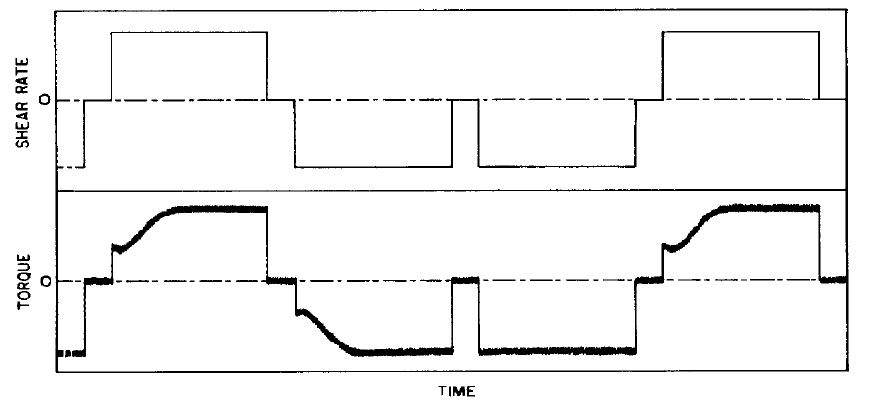
\includegraphics[width=10.6009cm,height=4.714cm]{GadalaExp.eps}\caption{Start and stop shear flow experiment;\break the torque would be proportional
to the shear stress, after\break Gadala-Maria and Acrivos \cite{Gadala80}}
\label{Fig 1}
\end{figure}\pagebreak


%EndExpansion



\section{General bulk suspension properties}


\subsection{Bulk stress and stresslet}

We now consider a representative volume $V=V_{p}\cup V_{f},$ which
is large enough to contain many particles but small enough so that
macroscopic variables hardly change on the scale $V^{1/3}$, i.e.
$a\ll V^{1/3}\ll L$. The existence of such representative volume
is taken as an assumption in most works dealing with properties of
an effective continuum (i.e. \textit{homogenization}). The effective
stress tensor seen from a macroscopic level is simply the volume-averaged
stress \cite{landau59}: 
\begin{equation}
\left\langle \mathbf{\sigma}\right\rangle =\frac{1}{V}\int_{V}\mathbf{\sigma}\ dV=\frac{1}{V}\int_{V_{f}}\mathbf{\sigma}dV+\frac{1}{V}\int_{V_{p}}\mathbf{\sigma}dV,
\end{equation}
where the angle brackets denote a volume-averaged quantity. With a
Newtonian solvent, the stress is a hydrostatic pressure plus an extra
stress proportional to the strain rate tensor $D_{ij}=\left(\partial u_{i}/\partial x_{j}+\partial u_{j}/\partial x_{i}\right)/2$
($\mathbf{u}$ is the imposed velocity vector):
\[
\mathbf{\sigma}(\mathbf{x})=-P\mathbf{I}+2\eta_{s}\mathbf{D}\equiv\mathbf{\sigma}^{(f)},\quad\mathbf{x}\in V_{f}.
\]

Thus: 
\[
\frac{1}{V}\int_{V_{f}}\mathbf{\sigma}dV=-\left\langle P\right\rangle \mathbf{I}+2\eta_{s}\left\langle \mathbf{D}\right\rangle -\frac{1}{V}\int_{V_{p}}\mathbf{\sigma}^{(f)}dV.
\]

Furthermore, in the absence of microinertia and the body force, the
micromechanics must satisfy the balance of momentum (using Cartesian
tensor notation) $\partial\sigma_{ij}/\partial x_{j}=0,$ which implies:
\[
\frac{\partial}{\partial x_{k}}\left(x_{i}\sigma_{kj}\right)=\sigma_{ij},
\]
and we find that: 
\begin{equation}
\frac{1}{V}\int_{V_{p}}\sigma_{ij}\ dV=\frac{1}{V}\int_{V_{p}}\frac{\partial}{\partial x_{k}}\left(x_{i}\sigma_{kj}\right)\ dV=\frac{1}{V}\int_{S_{p}}x_{i}t_{j}\ dS,
\end{equation}
where $t_{j}=\sigma_{kj}n_{k}$ is the traction vector and the divergence
theorem has been used to convert the volume integral into a surface
integral over the bounding surface $S_{p}$ of all the particles.
In addition, with the Newtonian solvent assumption and using the divergence
theorem: 
\begin{eqnarray*}
\frac{1}{V}\int_{V_{p}}\sigma_{ij}^{(f)}~dV & =&\frac{1}{V}\int_{V_{p}}\left[-P\delta_{ij}+\eta_{s}\left(\frac{\partial u_{i}}{\partial x_{j}}+\frac{\partial u_{j}}{\partial x_{i}}\right)\right]\ dV\\
 & =&-P_{1}\delta_{ij}+\frac{1}{V}\int_{S_{p}}\left[\eta_{s}\left(u_{i}n_{j}+u_{j}n_{i}\right)\right]\ dS~
\end{eqnarray*}
where $P_{1}$ is the scalar pressure. The average stress is thus
given by: 
\begin{equation}
\left\langle \sigma_{ij}\right\rangle =-P^{\prime}\delta_{ij}+\underset{\text{solvent}}{\underbrace{2\eta_{s}\left\langle D_{ij}\right\rangle }}+\underset{\text{particles}}{\underbrace{\frac{1}{V}\int_{S_{p}}\left\{ x_{i}t_{j}-\eta_{s}\left(u_{i}n_{j}+u_{j}n_{i}\right)\right\} \ dS}},
\end{equation}
consisting of a solvent contribution and a particle contribution;
$P^{\prime}$ is just a scalar pressure (the prime will be dropped
from hereon). The particle contribution can be decomposed into a symmetric
part and an antisymmetric part. The symmetric part is, in fact, the
sum of the \textit{stresslets} $\mathcal{S}_{ij}^{(p)}$ defined by
\cite{batchelor70}: 
\begin{equation}
\mathcal{S}_{ij}=\frac{1}{2}\int_{S_{p}}\left\{ x_{i}t_{j}+x_{j}t_{i}-2\eta_{s}\left(u_{i}n_{j}+u_{j}n_{i}\right)\right\} \ dS=\sum_{p}\mathcal{S}_{ij}^{(p)},\label{stresslet}
\end{equation}
and the antisymmetric part leads to the rotlet \cite{batchelor70}:
\begin{equation}
\mathcal{R}_{ij}=\frac{1}{2}\int_{S_{p}}\left(x_{i}t_{j}-x_{j}t_{i}\right)\ dS=\frac{1}{2}\sum_{p}\epsilon_{ijk}T_{k}^{(p)},
\end{equation}
where $T_{k}^{(p)}$ is the torque exerted on the particle $p$, $\varepsilon_{ijk}$
is the alternating tensor and the summation is over all particles
in the volume $V$. The particle-contributed stress is, therefore,
given by: 
\begin{equation}
\sigma_{ij}^{(p)}=\frac{1}{V}\sum_{p}\left(\mathcal{S}_{ij}^{(p)}+\frac{1}{2}\epsilon_{ijk}T_{k}^{(p)}\right).\label{p-stress}
\end{equation}


A more general approach for calculating stresslet for a general particle
based on singularity multipole expansion and/or Faxén theorem is detailed
in \cite{kim91}, with a parallel development in elasticity in \cite{phan-thien94}.


\subsection{Bulk dissipation}

Sometimes, it is desirable to compute the total rate of energy dissipation.
By considering a volume $V$ large enough to contain all the particles,
the total rate of energy dissipation in $V$ is thus:
\begin{equation}
\Phi=\int_{V}\sigma_{ij}D_{ij}\ dV=\int_{V}\frac{\partial}{\partial x_{j}}\left(\sigma_{ij}u_{i}\right)\ dV={\displaystyle \sum\limits _{p}}\int_{S_{p}}\sigma_{ij}u_{i}n_{j}\ dS.\label{375}
\end{equation}

The second equality comes from the balance of momentum, and the third
equality comes from an application of the divergence theorem, assuming
that the condition at infinity is quiescent (the bounding surface
of $V$ consists of particles' surfaces and surface at infinity).
For a system of rigid particles, the boundary condition on the surface
of a particle $p$ is that: 
\begin{equation}
\mathbf{u}=\mathbf{U}^{(p)}+\mathbf{\Omega}^{(p)}\times\mathbf{x},
\end{equation}
where $\mathbf{U}^{(p)}$ and $\mathbf{\Omega}^{(p)}$ are the translational
and rotation velocities of the particle, which can be taken outside
the integral in [\ref{375}], and the remaining integrals can
be identified with the force $\mathbf{F}^{(p)}$ and the torque $\mathbf{T}^{(p)}$
imparted by the particle $p$ to the fluid. Thus, the total rate of
energy dissipation is: 
\begin{equation}
\Phi=\sum_{p}\left(\mathbf{U}^{(p)}\cdot\mathbf{F}^{(p)}+\mathbf{\Omega}^{(p)}\cdot\mathbf{T}^{(p)}\right).
\end{equation}

Note also that for a system of rigid particles, the integral: 
\[
\int_{S_{p}}\left(\mathbf{un}+\mathbf{nu}\right)dS=\mathbf{0},
\]
since: 
\[
\int_{S_{p}}\mathbf{U}^{(p)}\mathbf{n}dS=\mathbf{0},\quad\int_{S_{p}}\left(\mathbf{\Omega}^{(p)}\times\mathbf{xn}+\mathbf{n\Omega}^{(p)}\times\mathbf{x}\right)dS=\mathbf{0},
\]
by applications of the divergence theorem.


\section{Dilute suspension of rigid spheres}


\subsection{Stresslet}

We now consider a dilute suspension of force- and torque-free monodispersed
spheres, of radius $a$ each, in an ambient uniform flow $\mathbf{U}$
superimposed by shear flow of velocity gradient $\mathbf{L}=\mathbf{D}+\mathbf{W,}$
where $\mathbf{D}$ is the strain rate tensor and $\mathbf{W}$, the
vorticity tensor. Dilute concentration means the volume fraction:
\begin{equation}
\phi=\nu\frac{4\pi a^{3}}{3}\ll1,
\end{equation}
where $\nu$ is the number density of the spheres. In this case, in
a representative volume $V$, we expect to find only one sphere in
isolation. Thus, the micromechanic problem consists of a single sphere
in an effectively unbounded fluid -- unbounded here means far away
from the particle concerned, but still not far enough to run into another
sphere. The relevant boundary conditions for this micromechanic problem
are: 
\begin{equation}
\mathbf{u}\left(\mathbf{x}\right)=\mathbf{U}+(\mathbf{D}+\mathbf{W})\cdot\mathbf{x},\quad\text{far from the particle, }\left\vert \mathbf{x}\right\vert \rightarrow\infty,
\end{equation}
and 
\begin{equation}
\mathbf{u}\left(\mathbf{x}\right)=\mathbf{V}+\mathbf{w}\cdot\mathbf{x},\quad\text{on the particle's surface, }\left\vert \mathbf{x}\right\vert =a.
\end{equation}

Here, $\left(\mathbf{V},\mathbf{w}\right)$ constitute a rigid body
motion of the particle, with $\mathbf{V}$ its translational motion
and $\mathbf{w}$ a skew-symmetric tensor such that $w_{ij}=-\epsilon_{ijk}\Omega_{k}$,
where $\mathbf{\Omega}$ is the angular velocity of the particle.
The solution to this unbounded flow problem can be generated from
Lamb's solution \cite{happel73}, or it can be synthesized from Stokes'
singular solution \cite{phan-thien94}: 
\begin{eqnarray}
\mathbf{u} & =&\mathbf{U}+\mathbf{L}\cdot\mathbf{x}+\frac{a^{3}}{x^{3}}\left(\mathbf{w}-\mathbf{W}\right)\cdot\mathbf{x}+\left(\frac{3a}{4x}+\frac{a^{3}}{4x^{3}}\right)(\mathbf{V}-\mathbf{U})-\frac{a^{5}}{x^{5}}\mathbf{D}\cdot\mathbf{x}\nonumber \\
& & +\ \frac{3a}{x^{3}}\left(1-\frac{a^{2}}{x^{2}}\right)(\mathbf{V}-\mathbf{U})\cdot\mathbf{xx}-\frac{5a^{3}}{2x^{5}}\left(1-\frac{a^{2}}{x^{2}}\right)\mathbf{D}:\mathbf{xxx},\label{sphere-sol}
\end{eqnarray}
and 
\begin{equation}
P=\frac{3}{2}\eta_{s}\frac{a}{x^{3}}(\mathbf{V}-\mathbf{U})\cdot\mathbf{x}-5\eta_{s}\frac{a^{3}}{x^{5}}\mathbf{D}:\mathbf{xx}.
\end{equation}

From this, the strain rate tensor and the stress can be calculated
leading to the traction on the surface of the sphere: 
\begin{equation}
\mathbf{t}=\mathbf{\sigma}\cdot\mathbf{n}|_{x=a}=-\frac{3\eta_{s}}{2a}(\mathbf{V}-\mathbf{U})-\frac{3\eta_{s}}{a}(\mathbf{w}-\mathbf{W})\cdot\mathbf{x}+5\frac{\eta_{s}}{a}\mathbf{D}\cdot\mathbf{x}.\label{traction}
\end{equation}

The force and the torque on the particle can be evaluated: 
\begin{equation}
\mathbf{F}=\int_{S}\mathbf{\sigma}\cdot\mathbf{n}\ dS=-6\pi\eta_{s}a(\mathbf{V}-\mathbf{U})
\end{equation}
and 
\begin{equation}
\mathbf{T}=\int_{S}\mathbf{x}\times\mathbf{\sigma}\cdot\mathbf{n}dS=-8\pi\eta_{s}a^{3}(\mathbf{\Omega}-\mathbf{\omega}),
\end{equation}
where $\omega_{i}=\frac{1}{2}\epsilon_{ijk}W_{jk}$ is the local vorticity
vector. Thus, if the particle is force-free and torque-free, then
it translates with $\mathbf{U}$ and spin with an angular velocity
of $\mathbf{\omega}$.

Returning now to the particle-contributed stress, [\ref{p-stress}],
\[
\left\langle \sigma_{ij}^{(p)}\right\rangle =\frac{1}{V}\sum_{p}\mathcal{S}_{ij}=\nu\mathcal{S}_{ij},
\]
where the stresslet is given in [\ref{stresslet}]. From [\ref{traction}],
and noting that
\[
\int_{S}\mathbf{x}\ dS=\mathbf{0},\quad\int_{S}\mathbf{xx}\ dS=\frac{4\pi a^{4}}{3}\mathbf{1},
\]
we find 
\[
\mathcal{S}_{ij}=\frac{1}{2}\int_{S}\left(x_{i}t_{j}+x_{j}t_{i}\right)\ dS=5\frac{\eta_{s}}{a}\int_{S}D_{ik}x_{k}x_{j}\ dS=5\eta_{s}\left(\frac{4\pi a^{3}}{3}\right)D_{ij}.
\]

Recall that the volume fraction of particles is $\phi=4\pi a^{3}\nu/3$;
the total effective stress, consisted of the solvent stress and the
particle-contributed stress, will now become: 
\begin{equation}
\left\langle \mathbf{\sigma}\right\rangle =-P\mathbf{1}+2\eta_{s}\left(1+\frac{5}{2}\phi\right)\mathbf{D},
\end{equation}
and consequently the dilute suspension is Newtonian, with a reduced
viscosity of:
\begin{equation}
\mu_{r}=\frac{\eta}{\eta_{s}}=1+\frac{5}{2}\phi.\label{einstein}
\end{equation}

This is the celebrated Einstein result \cite{einstein03}, who
arrived at the conclusion from the equality of the dissipation at
the microscale and the macroscale as described~by an effective Newtonian
viscosity. It is generally agreed that [\ref{einstein}] is quite
accurate at a volume fraction $\phi<0.02.$ Current research aims to
understand~moderate to concentrated suspensions, for both Newtonian
\cite{foss00, zarraga00, Pan10, dai13, phanthien14b}
and non-Newtonian suspensions \cite{lyon01, zarraga01, gleissle02,
tanner10}); not surprisingly, due to the complex nature of
the fluids, most of these studies are numerical modeling in nature.


\subsection{An exact poly-dispersed model}

Although the limitation on [\ref{einstein}] is quite severe,
it may be used to arrive at an exact theoretical construction for
a poly-dispersed suspension at an arbitrary volume fraction, which
could provide some guidance into an experimental correlation. The
process starts by adding a small infinitesimal volume $\Delta\phi$
of the particulate rigid phase of size $a.$ The effective medium
is Newtonian, and its viscosity is given by:
\begin{equation}
\eta^{\prime}=\eta_{s}\left(1+\frac{5}{2}\Delta\phi\right).
\end{equation}

To this effective Newtonian medium, another infinitesimal volume fraction
of particulate rigid phase, of  considerably larger size than that
of the previous step, is added. This process continues until a finite
volume fraction $0<\phi<1$ is built up. At an intermediate step,
denote the viscosity at volume fraction $\phi$ by $\eta.$ To a normalized
unit volume of this, we add a $\Delta\phi$ volume of a particulate
phase, of volume fraction $\Delta\phi/\left(1+\Delta\phi\right).$
This results in an effective Newtonian fluid of viscosity:
\[
\eta+d\eta=\eta\left(1+\frac{5}{2}\frac{\Delta\phi}{1+\Delta\phi}\right).
\]

Since in a volume $\left(1+\Delta\phi\right)$ of the suspension,
there has been a volume $\phi$ of the particulate phase, now augmented
by $\Delta\phi,$ the actual volume fraction has been increased by:
\[
d\phi=\frac{\phi+\Delta\phi}{1+\Delta\phi}-\phi=\frac{\Delta\phi}{1+\Delta\phi}\left(1-\phi\right),
\]
and, therefore, we can build up the following differential model for
the viscosity: 
\[
\frac{d\eta}{\eta}=\frac{5d\phi}{2\left(1-\phi\right)}
\]
which can be integrated, subjected to $\eta\left(\phi=0\right)=\eta_{s}$
to yield: 
\begin{equation}
\frac{\eta}{\eta_{s}}=\frac{1}{\left(1-\phi\right)^{5/2}}.\label{rigid-poly}
\end{equation}

This relation was proposed and investigated by Roscoe \cite{roscoe52}.
He noted that the relation works well for poly-dispersed suspensions
of spheres at low volume fraction; however, as the relation allows
for a maximum packing ratio of $\phi=1,$ he recommended that, at
high volume fraction, $\phi$ should be replaced by $\phi/\phi_{m},$
where $\phi_{m}\approx0.74$ for a better agreement with experimental
data.

This construction is called a \textit{differential scheme} in composite
materials \cite{norris85}, \cite{norris85b}. There have been several
results reported by Phan-Thien and Pham \cite{phan-thien97} for viscosity
and elasticity models of multiphase materials; the particulate phases
may be rigid, droplets and bubbles, or a combination of them. Recently,
Tanner \textit{et al}. \cite{tanner10} reported a differential scheme
for a weakly viscoelastic solvent.


\section{Dilute suspension of spherical droplets}

Small droplets (made up of an incompressible Newtonian fluid) do not
suffer significantly in their deformation and can be considered spherical
as they are transported in the flow. Their analysis is complicated
by the fact that the interior flow has to match with the exterior
flow on their surfaces, and the extra parameter:
\begin{equation}
\lambda=\frac{\eta_{d}}{\eta_{s}},
\end{equation}
the ratio of interior to exterior viscosity comes into play. Here,
the solution for a droplet is available from the literature, which
can be used in a similar manner to generate the stresslet. The readers
are referred to \cite{kim91} for an elegant treatment of Faxén theorem
leading to the main result that the suspension is Newtonian, with
an effective reduced viscosity of:
\begin{equation}
\mu_{r}=\frac{\eta}{\eta_{s}}=1+\frac{2+5\lambda}{2\left(1+\lambda\right)}\phi,
\end{equation}
which reduces to Einstein's relation when $\lambda\rightarrow\infty$
(for a rigid droplet suspension). For a dilute suspension of gas bubbles
($\lambda=0$),
\begin{equation}
\mu_{r}=\frac{\eta}{\eta_{s}}=1+\phi.
\end{equation}
\indent
Relations for poly-dispersed suspensions similar to [\ref{rigid-poly}]
are also available. For instance, a poly-dispersed suspension of droplets
of viscosity ratio $\lambda$, constructed in the manner of a differential
scheme, would have an effective viscosity implicitly given by:\vspace*{-3pt}
\begin{equation}
\phi=1-\mu_{r}^{-2/5}\left(\frac{2+5\lambda}{2\mu_{r}+5\lambda}\right)^{3/5}.
\end{equation}\vspace*{3pt}



\section{Dilute suspension of rigid spheroids}


\subsection{Jeffery's solution and stress rule}

For a dilute suspension of spheroids, a similar theory to the suspension
of spheres has been worked out by Leal and Hinch \cite{leal73} using
Jeffery's solution \cite{jeffery22}. Here, if $\mathbf{p}$ denotes
a unit vector directed along the major axis of the spheroid, then
Jeffery's solution states that: 
\begin{eqnarray}
\mathbf{\dot{p}} & =&\mathbf{W}\cdot\mathbf{p}+\frac{R^{2}-1}{R^{2}+1}\left(\mathbf{D}\cdot\mathbf{p}-\mathbf{D}:\mathbf{ppp}\right),\label{9.1}\\
 & =&\mathbf{L}\cdot\mathbf{p}-\frac{2}{R^{2}+1}\mathbf{D}\cdot\mathbf{p}-\frac{R^{2}-1}{R^{2}+1}\mathbf{D}:\mathbf{ppp}\nonumber 
\end{eqnarray}
where $R$ is the aspect ratio of the particle (major to minor diameter
ratio). The evolution of $\mathbf{p}$ is also referred to as Jeffery's
orbit. Usually, the effects of Brownian motion are also included as
white noise perpendicular to $\mathbf{p}$ on the right-hand side
of [\ref{9.1}], so as to preserve the unit length of $\mathbf{p}.$
Here, $\mathbf{L}=\mathbf{D}+\mathbf{W}$ is the velocity gradient,
where $\mathbf{D}$ is the strain rate and $\mathbf{W}$ is the vorticity
tensor.

To complete the constitutive description of the suspension, a stress
rule on how to calculate the stress from the evolving microstructure
(as represented by $\mathbf{p}$) must be provided. There have been
many paths to accomplish this goal. In the continuum path, we may
select a relevant structure tensor (for example, $\mathbf{pp}$) and
postulate that the stress is a functional of this structure tensor
and a kinematic measure (for example, the strain rate tensor). From
this general assumption, we can construct continuum models that satisfy
various principles that we know all physical models must follow, and
restrict them to behave in the manner required by the physics of the
micromechanics (for example, linear and instantaneous responses).
Notable contributions from this approach are given by Hand \cite{hand62}
and Ericksen \cite{ericksen60}. We can also build up models based
on a generic type of interactions, for example the spheres model of
Goddard and Miller \cite{goddard}, the transverse isotropic fiber
model of Folgar and Tucker \cite{folgar84} and the concentrated suspension
model of Phan-Thien \textit{et al}. \cite{phan-thien99}. We will
see more of this approach in this book. These models tend to mimic
certain aspects of the micromechanics provided by the more exact and
rigorous framework of dilute suspension of spheroids.

In the case of a dilute suspension of rigid spheroids, the stresslet
is expressed in terms of some elliptic integrals \cite{kim91}, which
can be extracted asymptotically to yield, for the particle-contributed
stress \cite{leal73}: 
\begin{eqnarray}
\mathbf{\sigma}^{(p)} & =&2\eta_{s}\phi\{A\mathbf{D}:\left\langle \mathbf{pppp}\right\rangle +B\left(\mathbf{D}\cdot\left\langle \mathbf{pp}\right\rangle +\left\langle \mathbf{pp}\right\rangle \cdot\mathbf{D}\right)\label{TIF}\\
& & +C\mathbf{D}+d_{R}F\left\langle \mathbf{pp}\right\rangle \},\nonumber 
\end{eqnarray}
where the angular brackets denote the ensemble average with respect
to the distribution function of $\mathbf{p}$ if stochastic noise
is used to model the Brownian interaction in [\ref{9.1}]; $A$,
$B$, $C$ and $F$ are some shape factors, and $d_{R}$ is the rotational
diffusivity. If the particles are large enough so that Brownian motion
can be ignored, then the last term, as well as the angular brackets,
can be omitted in [\ref{TIF}]. The asymptotic values of the shape
factors have been evaluated by Leal and Hinch \cite{leal73}; they
are given in Table \ref{table4.1}.%TCIMACRO{\TeXButton{B}{\begin{table}[tbp]}}%
%BeginExpansion
%EndExpansion%


%EndExpansion



\subsection{Jeffery's orbit}

Jeffery's equation is solved by: 
\begin{equation}
\mathbf{p}=\frac{\mathbf{Q}}{Q},
\end{equation}
where: 
\begin{equation}
\mathbf{\dot{Q}}=\mathcal{L}\cdot\mathbf{Q},\quad\mathcal{L}=\mathbf{L}-\frac{2}{R^{2}+1}\mathbf{D},\label{9.2}
\end{equation}
as can be verified directly, $\mathbf{\dot{Q}}=\mathbf{\dot{p}}Q+\mathbf{p}\dot{Q}.$
With $\mathbf{p}$ a unit vector, $\mathbf{\dot{p}\cdot p}=0,$ this
yields:
\begin{eqnarray*}
\dot{Q} & =&\mathbf{p}\cdot\mathbf{\dot{Q}}=Q\left(1-\frac{2}{R^{2}+1}\right)\mathbf{D}:\mathbf{pp}\\
 & =&Q\frac{R^{2}-1}{R^{2}+1}\mathbf{D}:\mathbf{pp.}
\end{eqnarray*}

\begin{table}[h]%\vspace*{-6pt}
\centering
\fontsize{9}{11}\selectfont
\begin{tabular}{|l|c|c|c|}
\hline 
Asymptotic  & $R\rightarrow\infty$  & $R=1+\delta,\;\delta\ll1$  & $R\rightarrow0$\tabularnewline
limit  & (rod-like)  & (near-sphere)  & (disk-like)\tabularnewline
\hline 
$A$  & $\dfrac{R^{2}}{2(\ln2R-1.5)}$  & $\dfrac{395}{147}\delta^{2}$  & $\dfrac{10}{3\pi R}+\dfrac{208}{9\pi^{2}}-2$\tabularnewline
 &  &  & \tabularnewline
$B$  & $\dfrac{6\ln2R-11}{R^{2}}$  & $\dfrac{15}{14}\delta-\dfrac{395}{588}\delta^{2}$  & $-\dfrac{8}{3\pi R}+1-\dfrac{128}{9\pi^{2}}$\tabularnewline
 &  &  & \tabularnewline
$C$  & 2  & $\dfrac{5}{2}\left(1-\dfrac{2}{7}\delta+\dfrac{1}{3}\delta^{2}\right)$  & $\dfrac{8}{3\pi R}$\tabularnewline
 &  &  & \tabularnewline
$F$  & $\dfrac{3R^{2}}{\ln2R-1/2}$  & $9\delta$  & $-\dfrac{12}{\pi R}$\tabularnewline
\hline 
\end{tabular}
\caption{Asymptotic values of the shape factors, $R$ is the aspect ratio of
the particle; $R\rightarrow\infty$ represents a rod-like particle
(a slender prolate spheroid, $R\approx1$ represents a near-sphere
particle and $R\rightarrow0$ represents a disk-like particle (flat
oblate spheroid) \label{table4.1}}\vspace*{-12pt}


%TCIMACRO{\TeXButton{E}{\end{table}}}%
%BeginExpansion
\end{table}


When this is substituted back to $\mathbf{\dot{p}}Q=\mathbf{\dot{Q}}-\mathbf{p}\dot{Q},$
we obtain:
\[
\mathbf{\dot{p}}Q=\left(\mathbf{L}-\frac{2}{R^{2}+1}\mathbf{D}\right)Q\mathbf{p}-Q\frac{R^{2}-1}{R^{2}+1}\mathbf{D}:\mathbf{ppp}
\]
leading to equation [\ref{9.1}]. The main advantage of this is
that we  only have to deal with a linear system [\ref{9.2}], instead
of the nonlinearity in [\ref{9.1}]. In addition, when Brownian
effects are considered, it may be less complicated by adding an unconstrained
stochastic process directly to [\ref{9.2}] -- stochastic process
adding to [\ref{9.1}] has to be constrained so as to preserve
the unit vector $\mathbf{p}.$

The rheological predictions of this constitutive equation have also
been considered by Hinch and Leal \cite{hinch72}. In essence, the
viscosity is shear thinning, the first normal stress difference is
positive, while the second normal stress difference is negative, but
of a smaller magnitude. The precise values depend on the aspect ratio
and the strength of the Brownian motion. The limit $R\rightarrow\infty$
corresponds to a slender particle (prolate spheroid of a large aspect
ratio $R$), and the rest of the discussion is pertinent to this limit.

In a start-up of a shear flow of shear rate $\dot{\gamma}$ (assumed
positive here), given an initial state for $\mathbf{p}_{0}=\mathbf{Q}_{0}/Q_{0}$
expressed as $\left\{ Q_{10},Q_{20},Q_{30}\right\} ,$ the solution
to [\ref{9.2}] is: 
\begin{fleqnarray}
Q_{1} & =&Q_{10}\cos\omega t+RQ_{20}\sin\omega t=\left(Q_{10}^{2}+R^{2}Q_{20}^{2}\right)^{1/2}\cos\left(\omega t-\vartheta\right)\nonumber \\
Q_{2} & =&Q_{20}\cos\omega t+R^{-1}Q_{10}\sin\omega t,=\left(R^{-2}Q_{10}^{2}+Q_{20}^{2}\right)^{1/2}\sin\left(\omega t-\vartheta\right)\\
Q_{3} & =&Q_{30},\nonumber 
\end{fleqnarray}%
and the frequency of the oscillation is: 
\begin{equation}
\omega=\frac{1}{2}\dot{\gamma}\sqrt{\zeta(2-\zeta)}=\frac{\dot{\gamma}R}{R^{2}+1},\;\;\;\vartheta=\tan^{-1}\frac{RQ_{20}}{Q_{10}},
\end{equation}
where $\zeta=2/\left(R^{2}+1\right).$ Thus, the particles tumble
along with the flow, with a period of $T=2\pi/\omega=2\pi(R^{2}+1)/\dot{\gamma}R=O\left(R/\dot{\gamma}\right)$,
spending most of their time aligned with the flow to within an angle
$O\left(R^{-1}\right)$ from the flow-vorticity plane. Then, it quickly
flips through the remaining orbit in a fraction $O\left(R^{-1}\right)$
of the period.%TCIMACRO{\FRAME{ftbphFU}{7.7792cm}{6.5371cm}{0pt}{\Qcb{Some Jeffery orbits at
%$R=20.$ Each orbit has a unique orbital constant. Orbit of $C_{j}=0$ reduces
%to a point on the vorticity axis; orbit $C_{j}=\infty$ is located on the
%flow-gradient plane.}}{\Qlb{JefferyOrbit}}{jefferyorbit.jpg}%
%{\special{ language "Scientific Word";  type "GRAPHIC";
%maintain-aspect-ratio TRUE;  display "USEDEF";  valid_file "F";
%width 7.7792cm;  height 6.5371cm;  depth 0pt;  original-width 13.361cm;
%original-height 11.2017cm;  cropleft "0";  croptop "1";  cropright "1";
%cropbottom "0";  filename 'JefferyOrbit.JPG';file-properties "XNPEU";}} }%
%BeginExpansion
\begin{figure}[ptbh]
\centering
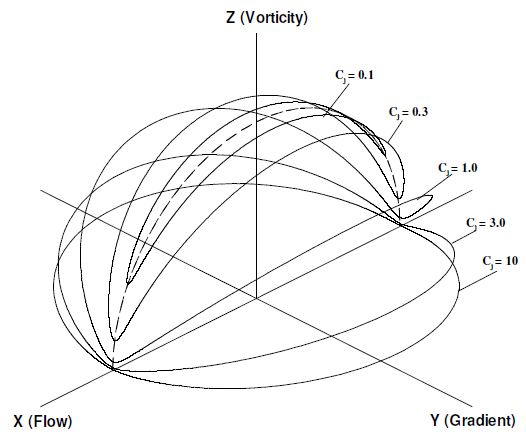
\includegraphics[width=8cm]{JefferyOrbit.eps}
\caption{Some Jeffery's orbits at $R=20.$ Each orbit has a unique orbital constant.
Orbit of $C_{j}=0$ reduces to a point on the vorticity axis; orbit
$C_{j}=\infty$ is located on the flow-gradient plane}
\label{JefferyOrbit}
\end{figure}


%EndExpansion


The projection of the orbit of $\mathbf{Q}$ on the flow-gradient
plane is an elliptic family:
\begin{equation}
\frac{Q_{1}^{2}\left(t\right)}{Q_{10}^{2}+R^{2}Q_{20}^{2}}+\frac{R^{2}Q_{2}^{2}\left(t\right)}{Q_{10}^{2}+R^{2}Q_{20}^{2}}=1
\end{equation}
at a distance $Q_{30}$ to the flow-gradient plane. This is usually
referred to as Jeffery's orbit. The initial position and the aspect
ratio of the particle completely determine the orbit of $\mathbf{Q}$
and, consequently, of $\mathbf{p}.$ The orbital constant $C_{j}$
is defined as:
\begin{equation}
C_{j}=\frac{\left(Q_{10}^{2}+R^{2}Q_{20}^{2}\right)^{1/2}}{RQ_{30}}=\frac{\left(Q_{1}^{2}+R^{2}Q_{2}^{2}\right)^{1/2}}{RQ_{3}}=\frac{\left(p_{1}^{2}+R^{2}p_{2}^{2}\right)^{1/2}}{Rp_{3}}.
\end{equation}

To avoid singular values, a modified orbital constant $C_{b}=C_{j}/\left(1+C_{j}\right),$\break
$0<C_{b}<1,$ is sometimes used.


The suspension viscometric properties are recorded below:

The reduced viscosity: 
\begin{equation}
\frac{\left\langle \sigma_{12}\right\rangle }{\eta_{s}\dot{\gamma}}=\mu_{r}=1+\left\langle 2Ap_{1}^{2}p_{2}^{2}+B\left(p_{1}^{2}+p_{2}^{2}\right)+C\right\rangle \phi,
\end{equation}
the reduced first normal stress difference: 
\begin{equation}
\frac{N_{1}}{\eta_{s}\dot{\gamma}}=2A\left\langle p_{1}p_{2}\left(p_{1}^{2}-p_{2}^{2}\right)\right\rangle \phi,
\end{equation}
and the reduced second normal stress difference: 
\begin{equation}
\frac{N_{2}}{\eta_{s}\dot{\gamma}}=2\left\langle p_{1}p_{2}\left(Ap_{2}^{2}+B\right)\right\rangle \phi.
\end{equation}

It has been known through simulation that $\left\langle p_{1}p_{2}\right\rangle $
is negative in shear flow, and consequently $N_{2}$ would be negative,
while $N_{1}$ can be either negative or positive. Note also that
all the viscometric functions are proportional to the shear rate (strictly
speaking, normal stress differences are proportional to the absolute
value of the shear rate).

In the start-up of an elongational flow with a (positive) elongational
rate $\dot{\gamma}$, the solution for Jeffery's orbit is: 
\begin{eqnarray}
Q_{1} & =&Q_{10}\exp\left\{ (1-\zeta)\dot{\gamma}t\right\} ,\nonumber \\
Q_{2} & =&Q_{20}\exp\left\{ -\frac{1}{2}(1-\zeta)\dot{\gamma}t\right\} ,\\
Q_{3} & =&Q_{30}\exp\left\{ -\frac{1}{2}(1-\zeta)\dot{\gamma}t\right\} ,\nonumber 
\end{eqnarray}
so that the particle is quickly aligned with the flow in a time scale
$O(\dot{\gamma}^{-1})$. The stress can be calculated and, in particular,
the reduced elongational viscosity of the suspension is:
\begin{equation}
\frac{N_{1}}{\eta_{s}\dot{\gamma}}=\mu_{re}=3+\left(2A+2B+C\right)\phi\approx\frac{\phi R^{2}}{\ln2R-1.5}.\label{8.21}
\end{equation}

For a dilute suspension of rod-like particle:
\begin{equation}
\mu_{re}\approx3+\frac{\phi R^{2}}{\ln2R-1.5},
\end{equation}
suggesting an $O\left(R^{2}\right)$ dependence of the elongational
viscosity on the aspect ratio. However, the dilute assumption means
that the volume fraction is low enough so that a particle can rotate
freely without any hindrance from its nearby neighbors. The distance
$\Delta$ between any two particles must therefore satisfy $l<\Delta$,
where $l$ is the length of a particle of diameter $d$, so that a
volume of $l^{3}$ contains only one particle. The volume fraction,
therefore, satisfies: 
\[
\phi\sim\frac{d^{2}l}{\Delta^{3}},\quad\phi R^{2}=\frac{l^{3}}{\Delta^{3}}<1.
\]

Thus, the reduced elongational viscosity is only $O(1)$ in the dilute
limit, and not $O(R^{2})$. Jeffery's solution may be used for a rod-like
particle when the aspect ratio $R$ has to be replaced by an effective
aspect ratio, $R_{e}\approx0.7R$ \cite{cox71}.

As the concentration increases, we get subsequently into the semi-dilute
regime ($1<\phi R^{2}<R$), the concentrated regime ($\phi R>1$ )
and the liquid crystalline solution ($\phi R\gg1$). In the concentrated
regime, where the average distance between fibers is less than a fiber
diameter, the fibers cannot rotate independently except around their
symmetry axes. Any motion of the fiber must necessarily involve a
cooperative motion of surrounding fibers. The readers are referred
to \cite{doi88} for more details. Later chapters (Chapters 4--5) deal with
the modeling at non-dilute concentrations.


\Remark{As the concentration increases, we get subsequently into the semi-dilute
regime ($1<\phi R^{2}<R$), the concentrated regime ($\phi R>1$ )
and the liquid crystalline solution ($\phi R\gg1$). In the concentrated
regime, where the average distance between fibers is less than a fiber
diameter, the fibers cannot rotate independently except around their
symmetry axes. Any motion of the fiber must necessarily involve a
cooperative motion of surrounding fibers. The readers are referred
to \cite{doi88} for more details. Later chapters (Chapters 4--5) deal with
the modeling at non-dilute concentrations.}

\Theorem{As the concentration increases, we get subsequently into the semi-dilute
regime ($1<\phi R^{2}<R$), the concentrated regime ($\phi R>1$ )
and the liquid crystalline solution ($\phi R\gg1$). In the concentrated
regime, where the average distance between fibers is less than a fiber
diameter, the fibers cannot rotate independently except around their
symmetry axes. Any motion of the fiber must necessarily involve a
cooperative motion of surrounding fibers. The readers are referred
to \cite{doi88} for more details. Later chapters (Chapters 4--5) deal with
the modeling at non-dilute concentrations.}

\Important{As the concentration increases, we get subsequently into the semi-dilute
regime ($1<\phi R^{2}<R$), the concentrated regime ($\phi R>1$ )
and the liquid crystalline solution ($\phi R\gg1$). In the concentrated
regime, where the average distance between fibers is less than a fiber
diameter, the fibers cannot rotate independently except around their
symmetry axes. Any motion of the fiber must necessarily involve a
cooperative motion of surrounding fibers. The readers are referred
to \cite{doi88} for more details. Later chapters (Chapters 4--5) deal with
the modeling at non-dilute concentrations.}

\begin{encadre}

As the concentration increases, we get subsequently into the semi-dilute
regime ($1<\phi R^{2}<R$), the concentrated regime ($\phi R>1$ )
and the liquid crystalline solution ($\phi R\gg1$). In the concentrated
regime, where the average distance between fibers is less than a fiber
diameter, the fibers cannot rotate independently except around their
symmetry axes. Any motion of the fiber must necessarily involve a
cooperative motion of surrounding fibers. The readers are referred
to \cite{doi88} for more details. Later chapters (Chapters 4--5) deal with
the modeling at non-dilute concentrations.


As the concentration increases, we get subsequently into the semi-dilute
regime ($1<\phi R^{2}<R$), the concentrated regime ($\phi R>1$ )
and the liquid crystalline solution ($\phi R\gg1$). In the concentrated
regime, where the average distance between fibers is less than a fiber
diameter, the fibers cannot rotate independently except around their
symmetry axes. Any motion of the fiber must necessarily involve a
cooperative motion of surrounding fibers. The readers are referred
to \cite{doi88} for more details. Later chapters (Chapters 4--5) deal with
the modeling at non-dilute concentrations.


As the concentration increases, we get subsequently into the semi-dilute
regime ($1<\phi R^{2}<R$), the concentrated regime ($\phi R>1$ )
and the liquid crystalline solution ($\phi R\gg1$). In the concentrated
regime, where the average distance between fibers is less than a fiber
diameter, the fibers cannot rotate independently except around their
symmetry axes. Any motion of the fiber must necessarily involve a
cooperative motion of surrounding fibers. The readers are referred
to \cite{doi88} for more details. Later chapters (Chapters 4--5) deal with
the modeling at non-dilute concentrations.


As the concentration increases, we get subsequently into the semi-dilute
regime ($1<\phi R^{2}<R$), the concentrated regime ($\phi R>1$ )
and the liquid crystalline solution ($\phi R\gg1$). In the concentrated
regime, where the average distance between fibers is less than a fiber
diameter, the fibers cannot rotate independently except around their
symmetry axes. Any motion of the fiber must necessarily involve a
cooperative motion of surrounding fibers. The readers are referred
to \cite{doi88} for more details. Later chapters (Chapters 4--5) deal with
the modeling at non-dilute concentrations.


As the concentration increases, we get subsequently into the semi-dilute
regime ($1<\phi R^{2}<R$), the concentrated regime ($\phi R>1$ )
and the liquid crystalline solution ($\phi R\gg1$). In the concentrated
regime, where the average distance between fibers is less than a fiber
diameter, the fibers cannot rotate independently except around their
symmetry axes. Any motion of the fiber must necessarily involve a
cooperative motion of surrounding fibers. The readers are referred
to \cite{doi88} for more details. Later chapters (Chapters 4--5) deal with
the modeling at non-dilute concentrations.
\end{encadre}
\encadrecaption{Caption}

\bibliographystyle{agsm}
\bibliography{chapter_1}
%\def\pagesname{pp.~}
%\def\numbername{no.~}
%\def\pagename{p.~}

%\begin{thebibliography}{A.N~85}
%
%\bibitem[BAT~70]{batchelor70} \textsc{Batchelor G.}, \guilo{}The stress system in a suspension of force-free particles\guilf{},
% \textit{Journal of Fluid Mechanics}, \volumename{}41, \pagesname
%545--570, 1970.
%
%\bibitem[COX~71]{cox71} \textsc{Cox R.},  ``The motion of long slender bodies in a viscous fluid. Part 2. Shear flow'', {\it Journal of Fluid Mechanics}, \volumename{}45, \pagesname 625--657, 1971.
%
%\bibitem[DAI~13]{dai13} \textsc{Dai S.-C.}, \textsc{Bertevas E.},
%\textsc{Qi F.} \textit{et al}., \guilo{}{Viscometric functions
%for noncolloidal sphere suspensions with Newtonian matrices}\guilf{},
% \textit{{Journal of Rheology}}, \volumename{}{57},
%\numbername{}{2}, \pagesname {493--510}, {2013}.
%
%\bibitem[DOI~88]{doi88} \textsc{Doi M.}\andname{}\textsc{Edwards
%S.}, \textit{The Theory of Polymer Dynamics},  Oxford University
%Press, Oxford, 1988.
%
%\bibitem[EIN~56]{einstein03} \textsc{Einstein A.}, \textit{Investigations
%on the Theory of the Brownian Movement},  {\sc Fürth R}. (ed.), Dover Publications, Inc., 
%New York, 1956.
%
%\bibitem[ERI~60]{ericksen60} {\sc Ericksen J.}, ``Transversely isotropic fluids'', {\it Kolloid-Zeischrift}, 
%\volumename{}173,\break \pagesname 117--122, 1960.
%
%\bibitem[FOL~84]{folgar84} \textsc{Folgar F.}\andname{}\textsc{Tucker
%C.},  ``Orientation behavior of fibers in concentrated suspensions'', {\it Journal of Reinforced Plasitcs and Composites}, \volumename{}3,
%\pagesname 98--119, 1984.
%
%\bibitem[FOS~00]{foss00} \textsc{Foss D.}\andname{}\textsc{Brady
%J.}, ``Structure, diffusion and rheology of Brownian suspensions by Stokesian  Dynamics simulation'', {\it Journal of Fluid Mechanics},
%\volumename{}407, \pagesname 167--200, 2000.
%
%\bibitem[GAD~80]{Gadala80} \textsc{Gadala-Maria F.}\andname{}\textsc{Acrivos
%A.}, \guilo{}Shear-induced structure in a concentrated suspension
%of solid spheres\guilf{},  \textit{Journal of Rheology},
%\volumename{}24, \numbername{}6, \pagesname 799--814, 1980.
%
%\bibitem[GOD~67]{goddard} \textsc{Goddard J.}\andname{}\textsc{Miller
%C.}, ``Non-linear effects in the rheology of dilute suspensions'', {\it Journal of Fluid Mechanics},  \volumename{}28, \pagesname 657--763, 1967.
%
%\bibitem[HAN~61]{hand62} \textsc{Hand G.}, ``A theory of dilute suspensions'', {\it Archive Rational Mechanics and Analyses}, \volumename{}7, \pagesname 81--86, 1961.
%
%\bibitem[HAP~73]{happel73} \textsc{Happel J.}\andname{}\textsc{Brenner
%H.}, \textit{Low Reynolds Number Hydrodynamics},  Noordhoff
%International Publishing, Leyden, 1973.
%
%\bibitem[HIN~72]{hinch72} \textsc{Hinch E.}\andname{}\textsc{Leal
%L.}, ``The effect of Brownian motion on the rheological properties of a suspension of non-spherical particles'', {\it Journal of Fluid Mechanics}, \volumename{}52,\break \pagesname
%683--712, 1972.
%
%\bibitem[JEF~22]{jeffery22} \textsc{Jeffery G.}, ``The motion of ellipsoidal particles immersed in viscous fluid'', {\it Proceedings of the Royal Society of London A}, \volumename{}102, \pagesname 161--179, 1922.
%
%\bibitem[KIM~91]{kim91} \textsc{Kim S.,~Karrila S.}, \textit{Microhydrodynamics:
%Principles and Selected Applications},  Butterworth and
%Heinemann, Boston, 1991.
%
%\bibitem[LAN~59]{landau59} \textsc{Landau L.}\andname{}\textsc{Lifshitz
%E.}, \textit{Fluid Mechanics},  Pergamon Press, New York,
%1959.
%
%\bibitem[LEA~73]{leal73} \textsc{Leal L.}\andname{}\textsc{Hinch
%E.}, ``Theoretical studies of a suspension of rigid particles affected by Brownian couples'',  \textit{Rheologica Acta}, \volumename{}12, \pagesname
%127--132, 1973.
%
%\bibitem[LIN~14]{phanthien14b} \textsc{Lin Y.}, \textsc{Phan-Thien
%N.}\andname{}\textsc{Khoo B.C.}, \guilo{}Normal stress differences
%behavior of polymeric particle suspension in shear flow\guilf{},
% \textit{Journal of Rheology}, \volumename{}58, \numbername{}1,\break
%\pagesname 223--235, 2014.
%
%\bibitem[LYO~01]{lyon01} \textsc{Lyon M.K.}, \textsc{Mead D.W.},
%\textsc{Elliott R.E.}\textit{ et al.}, \guilo{}Structure formation
%in moderately concentrated viscoelastic suspensions in simple shear
%flow\guilf{},  \textit{Journal of Rheology}, \volumename{}45,
%\numbername{}4, \pagesname 881--890, 2001.
%
%\bibitem[MAL~02]{gleissle02} \textsc{Mall-Gleissle S.}, \textsc{Gleissle
%W.}, \textsc{McKinley G.} \textit{et al.}, \guilo{}{The normal
%stress behaviour of suspensions with viscoelastic matrix fluids}\guilf{},
% \textit{{Rheologica Acta}}, \volumename{}{41}, nos. {1--2},
%\pagesname {61--76}, {2002}.
%
%\bibitem[MET~85]{metzner85} \textsc{Metzner A.B.}, \guilo{}Rheology
%of suspensions in polymeric liquids\guilf{},  \textit{Journal
%of Rheology}, \volumename{}29, \numbername{}6, \pagesname 739--775,
%1985.
%
%\bibitem[MEW~12]{Mewis} \textsc{Mewis J.}\andname{}\textsc{Wagner
%N.}, \textit{Colloidal Suspension Rheology},  Cambridge
%University Press, New York, 2012.
%
%\bibitem[MOR~09]{Morris} \textsc{Morris J.}, ``A review of microstructure in concentrated suspensions and its implications for rheology and bulk flow'',
% \textit{Rheologica Acta}, \volumename{}48, \pagesname
%909--923, 2009.
%
%\bibitem[NOR~85a]{norris85} \textsc{Norris A.}, ``A differential scheme for the effective moduli of composites'', {\it Mechanics of Materials}, \volumename{}4, \pagesname 1--16, 1985.
%
%\bibitem[NOR~85b]{norris85b} \textsc{Norris A.N., Callegari A.J.}\andname{}\textsc{Sheng
%P.}, ``A generalised differential effective medium theory'', {\it Journal of Mecahnics and Physics of Solids}, \volumename{}33,
%\pagesname 525--543, 1985.
%
%\bibitem[PAN~10]{Pan10} \textsc{Pan W.}, \textsc{Caswell B.}\andname{}\textsc{Karniadakis
%G.~E.}, \guilo{}{Rheology, microstructure and migration in Brownian
%colloidal suspensions}\guilf{},  \textit{{Langmuir}},
%\volumename{}{26}, \numbername{}{1}, \pagesname {133--142},
%{2010}.
%
%\bibitem[PHA~94]{phan-thien94} \textsc{Phan-Thien N.}\andname{}\textsc{Kim
%S.}, \textit{Microstructure in Elastic Media Principles and Computational
%Methods},  Oxford University Press, New York, 1994.
%
%\bibitem[PHA~97]{phan-thien97} \textsc{Phan-Thien N.}\andname{}\textsc{Pham
%D.}, \guilo{}Differential multiphase models for polydispersed suspensions
%and particulate solids\guilf{},  \textit{Journal of Non-Newtonian
%Fluid Mechanics}, \volumename{}72, nos. 2--3, \pagesname
%305--318, 1997.
%
%\bibitem[PHA~99]{phan-thien99} \textsc{Phan-Thien N.}, \textsc{Fan
%X.-J.}\andname{}\textsc{Khoo B.C.}, ``A new constitutive model for monodispersed suspensions
%of spheres at high concentrations'',  \textit{Rheologica
%Acta}, \volumename{}38, \pagesname 297--304, 1999.
%
%\bibitem[ROS~52]{roscoe52} \textsc{Roscoe R.}, ``The viscosity of suspensions of rigid spheres'', {\it British Journal of Applied Physics}, \volumename{}3, \pagesname 267--269, 1952.
%
%\bibitem[TAN~10]{tanner10} \textsc{Tanner R.I.}, \textsc{Qi F.}\andname{}\textsc{Housiadas
%K.D.}, \guilo{}{A differential model for the rheological properties
%of concentrated suspensions with weakly viscoelastic matrices}\guilf{},
% \textit{{Rheologica Acta}}, \volumename{}{49}, \numbername{}{2},
%\pagesname {169--176}, {2010}.
%
%\bibitem[ZAR~00]{zarraga00} \textsc{Zarraga I.E.}, \textsc{Hill
%D.A.}\andname{}\textsc{Leighton D.~T.}, \guilo{}The characterization
%of the total stress of concentrated suspensions of noncolloidal spheres
%in Newtonian fluids\guilf{},  \textit{Journal of Rheology},
%\volumename{}44, \numbername{}2, \pagesname 185--220, 2000.
%
%\bibitem[ZAR~01]{zarraga01} \textsc{Zarraga I.E.}, \textsc{Hill
%D.A.}\andname{}\textsc{Leighton D.T.}, \guilo{}Normal stresses
%and free surface deformation in concentrated suspensions of noncolloidal
%spheres in a viscoelastic fluid\guilf{},  \textit{Journal
%of Rheology}, \volumename{}45, \numbername{}5, \pagesname 1065--1084,
%2001.
%
%\end{thebibliography}


\part{Part title}

\chapter*{Introduction}

As the concentration increases, we get subsequently into the semi-dilute
regime ($1<\phi R^{2}<R$), the concentrated regime ($\phi R>1$ )
and the liquid crystalline solution ($\phi R\gg1$). In the concentrated
regime, where the average distance between fibers is less than a fiber
diameter, the fibers cannot rotate independently except around their
symmetry axes. Any motion of the fiber must necessarily involve a
cooperative motion of surrounding fibers. The readers are referred
to \cite{doi88} for more details. Later chapters (Chapters 4--5) deal with
the modeling at non-dilute concentrations.

\appendix
\chapter{Appendix title}

As the concentration increases, we get subsequently into the semi-dilute
regime ($1<\phi R^{2}<R$), the concentrated regime ($\phi R>1$ )
and the liquid crystalline solution ($\phi R\gg1$). In the concentrated
regime, where the average distance between fibers is less than a fiber
diameter, the fibers cannot rotate independently except around their
symmetry axes. Any motion of the fiber must necessarily involve a
cooperative motion of surrounding fibers. The readers are referred
to \cite{doi88} for more details. Later chapters (Chapters 4--5) deal with
the modeling at non-dilute concentrations.


\vfill\pagebreak
\
\thispagestyle{empty}
\end{document} 
